\begin{figure}
  \centering
	
	
  \hspace*{\fill}
	\subfigure[]{\label{subfig:2a}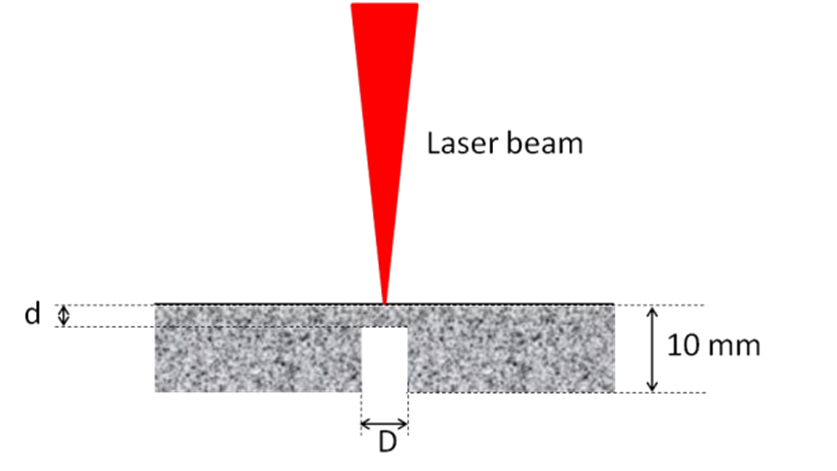
\includegraphics[width=0.3\linewidth]{./Figure/Figure2/a.png}}\hfill
	\subfigure[]{\label{subfig:2b}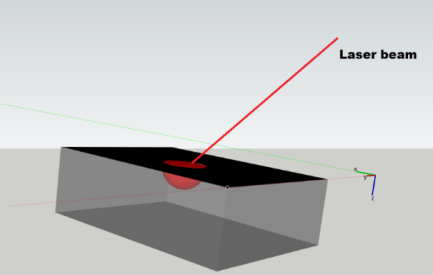
\includegraphics[width=0.3\linewidth]{./Figure/Figure2/b.png}} 
	\hspace*{\fill} \\ \hspace*{\fill}
	\subfigure[]{\label{subfig:2c}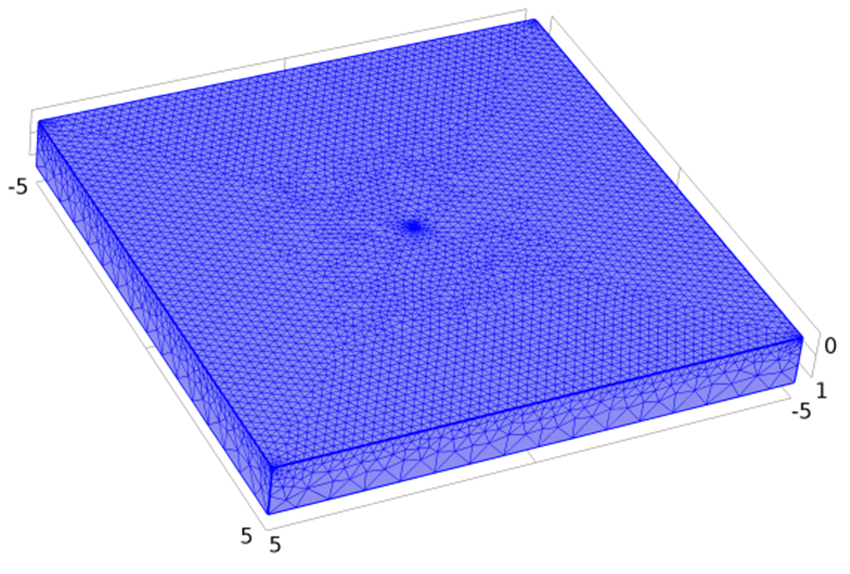
\includegraphics[width=0.3\linewidth]{./Figure/Figure2/c.png}}\hfill
	\subfigure[]{\label{subfig:2d}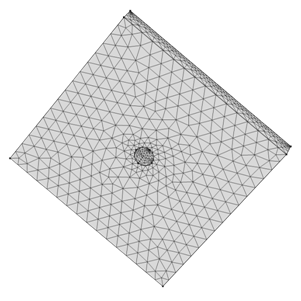
\includegraphics[width=0.3\linewidth]{./Figure/Figure2/d.png}}
	\hspace*{\fill}
    
	
		\caption{(a) Cross-sectional view of the geometry - (b) 3D Thermal response to a laser 
	excitation - (c) Geometry and meshing (front side), dimensions appears in cm  - (d) 
	Geometry and meshing (back side).}
  \label{fig:2}
\end{figure}
